
\documentclass[../summary.tex]{subfiles}

\begin{document}
	
	\section{Energie rechtvaardigheid}
	\subsection{Energie transitie}
	
	De \textbf{energietransitie} heeft enerzijds een hele hoop \textbf{technische uitdagingen}. We moeten er bijvoorbeeld voor zorgen dat we elektrolyse kunnen doen op een manier die genoeg energie-efficiënt is. We hebben nucleair afval dat we ergens moeten opslaan. We maken gebruik van zonnepanelen, maar de zon schijnt niet altijd, dus we moeten het elektriciteitsnet balanceren aangezien de stroomproductie zeer variabel is. Dit zijn allemaal hele lastige technologische uitdagingen. \\
	\\
	Aan de andere kant zijn er ook \textbf{sociale uitdagingen} van de energietransitie. Een voorbeeld hiervan zijn de extreem hoge energieprijzen. In het geval van armoede, energiearmoede bijvoorbeeld. Energie-infrastructuur moet ook ergens staan en mensen hebben dat het liefst niet in hun buurt. Hierdoor ontstaan er protesten die dan meestal gaan over het feit dat mensen erop tegen zijn dat de energie-infrastructuur door hun achtertuin moet lopen. We hebben daarnaast ook allerlei materialen nodig voor het maken van windmolens, zonnepanelen enzovoort. Die materialen komen heel vaak van plaatsen en gemeenschappen waar arbeidsomstandigheden zeer slecht zijn. Tenslotte hebben we heel veel infrastructuur nodig die soms door natuurreservaten lopen om de energie bij de gebruikers te krijgen, maar dit is voor de natuur en de mensen daar niet geweldig. Dit soort problemen zijn minstens zo groot als de technologische aspecten. 
	
	\subsection{Verdelen van het werk}
	
	Hoe moeten de technische en sociale uitdagingen verdeeld worden?  Er zijn drie mogelijke opvattingen mogelijk:

	\begin{description}
		\item[Separatisme] De technische zaken worden overgelaten aan ingenieurs, terwijl de niet-technische zaken worden opgelost door anderen zoals filosofen en politici.
		\item [Technocratie] Ingenieurs beslissen alles. Zij lossen zowel de technische en sociale challenges op.
		\item [Klokkenluider] Nog dikkere schijterij 
	\end{description}
	
	\subsubsection{Probleem van technocratie}
	
	Ingenieurs begrijpen wellicht niet alle perspectieven. De technocratie kan als \textbf{paternalistisch} en \textbf{ondemocratisch} beschouwd worden, omdat \textbf{ingenieurs beperkt zijn tot hun eigen achtergrond en perspectief}. Dit beperkte standpunt kan leiden tot een gebrek aan representatie van diverse perspectieven. Daarnaast \textbf{zou het ondemocratisch zijn als één groep alle beslissingen neemt}. De technocratie wordt dus als niet de beste oplossing gezien.
	
	
	\newpage
		
	\subsubsection{Separatisme}
	Bij separatisme treden er \textbf{twee problemen} op.
	\begin{description}
		\item[Hired Gun] Iemand die betaald wordt om technologie te ontwikkelen zonder verantwoordelijkheid te nemen voor de ethische implicaties ervan. Dit probleem kan relevant  zijn voor toekomstige ingenieurs, die mogelijk geconfronteerd worden met de keuze om technologieën te ontwikkelen waar ze niet volledig achter staan.
	\end{description}
	Een voorbeeld hiervan is \textbf{Wernher von Braun}, hij was een hired gun, een ingenieur die tijdens het nazisme in Duitsland werkte en later naar de Verenigde Staten ging om technologische ontwikkelingen te bevorderen. "Once the rockets go up, who cares where they come down, that's not my department." is zijn bekendste quote.
	
	\begin{description}
		\item[Is separatisme mogelijk?] Dit kan uitgelegd worden door middel van volgend voorbeeld.
	\end{description}
	Enerzijds heb je \textbf{Joseph Pitt} die zegt: \textbf{`Guns don't kill people, people kill people'}. Hiermee beweerd hij dat technologische artefacten geen waarden hebben of bevatten. Technologie is neutraal. Wij bepalen hoe we ze gebruiken. Dit kan worden gelinkt aan de \textbf{`Value Neutrality Thesis (VNT)'} en laat zien dat \textbf{separatisme mogelijk} is.\\
	\\
	Aan de andere kant heb je \textbf{Langdon Winner} die zegt: \textbf{`Actually, Guns do kill people'}. Hij beweert dus dat \textbf{technologische artefacten} wel degelijk \textbf{politiek geladen} kunnen zijn. Hij illustreert dit met het voorbeeld van bruggen ontworpen door architect Robert Moses in New York, die met opzet te laag waren voor bussen, waardoor vooral autobezitters toegang kregen tot bepaalde gebieden. Winner benadrukt dat technologieën niet neutraal zijn en inherent waarden bevatten, zoals in dit geval een racistische geladen. Hierdoor is \textbf{separatie dus niet mogelijk}.\\
	\\
	\textbf{Pitt} vindt het idee van waarden in technologische objecten belachelijk. Hij \textbf{vraagt waar die waarden dan zouden zitten - in welke steen, in welke hoogte?} Hij betoogt dat technologie niet intrinsiek waarden bevat en dat mensen verantwoordelijkheid moeten nemen voor hun handelingen. Hij \textbf{verwerpt het idee dat technologieën onethisch gedrag veroorzaken}, en benadrukt dat het de mensen zijn die verantwoordelijk zijn voor hun acties.\\
	\\
	De nuance in deze kwestie wordt benadrukt door \textbf{Michael Klenk}. Klenk introduceert het concept van \textbf{`affordances'} en stelt dat ingenieurs intenties en waarden hebben die vaak het ontwerp van een artefact beïnvloeden. Dit bepaalt op zijn beurt vaak hoe het artefact wordt gebruikt, hoewel de relatie niet strikt deterministisch is. Klenk legt uit dat artefacten bepaalde handelingen waarschijnlijker maken dan andere, vergelijkbaar met hoe een knop de neiging heeft om mensen in de richting van indrukken te sturen.
	
	\begin{figure}[H]
		\centering
		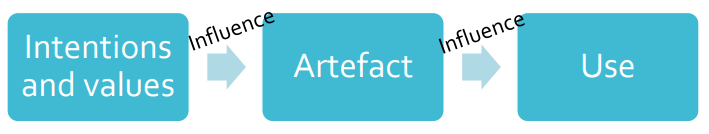
\includegraphics[width=0.7\linewidth]{../images/affordances}
		\caption{Hoe intenties en waardes het gebruik van een artefact beïnvloeden}
		\label{fig:affordances}
	\end{figure}
	
	\ \\
	Klenk's perspectief impliceert dat er \textbf{wel degelijk waarden in een artefact worden ingebracht door de ingenieur}, wat de vraag oproept over de verantwoordelijkheid van ingenieurs bij het creëren van technologieën. Als de intenties en waarden van de ingenieur op de een of andere manier in het artefact terechtkomen, suggereert dit dat het \textbf{niet volledig mogelijk} is \textbf{om sociale en technologische waarden te scheiden}. Dit werpt vragen op over de verantwoordelijkheid van degenen die technologieën ontwikkelen en of het idee van separatisme wel haalbaar is als waarden daadwerkelijk in de artefacten worden ingebed.
	
	\subsubsection{Technocratie}
	
	
	
\end{document}